%-----------------------------------------------------------------------
% Functional Programming 4
% John O'Donnell, Wim Vanderbauwhede
% University of Glasgow
%-----------------------------------------------------------------------

\documentclass{beamer}
\usepackage{jtodlecseriesFP4}
%include polycode.fmt
%format alpha = "\alpha"
%format ~> = "\leadsto "

% Identify this presentation
\SetPresentationTitle
  {Text Input/Output}
  {Text Input/Output}
\SetPresentationNumber
  {3}
\SetPresentationDate 
  {Week 2-1}
  {Week 2-1}

%-----------------------------------------------------------------------
% Beginning

\begin{document}

\begin{frame}[fragile]
  \PresentationTitleSlide
\end{frame}

\begin{frame}[fragile]
  \frametitle{Topics}
  \tableofcontents
\end{frame}
%-----------------------------------------------------------------------
\begin{frame}[fragile]
\begin{center}
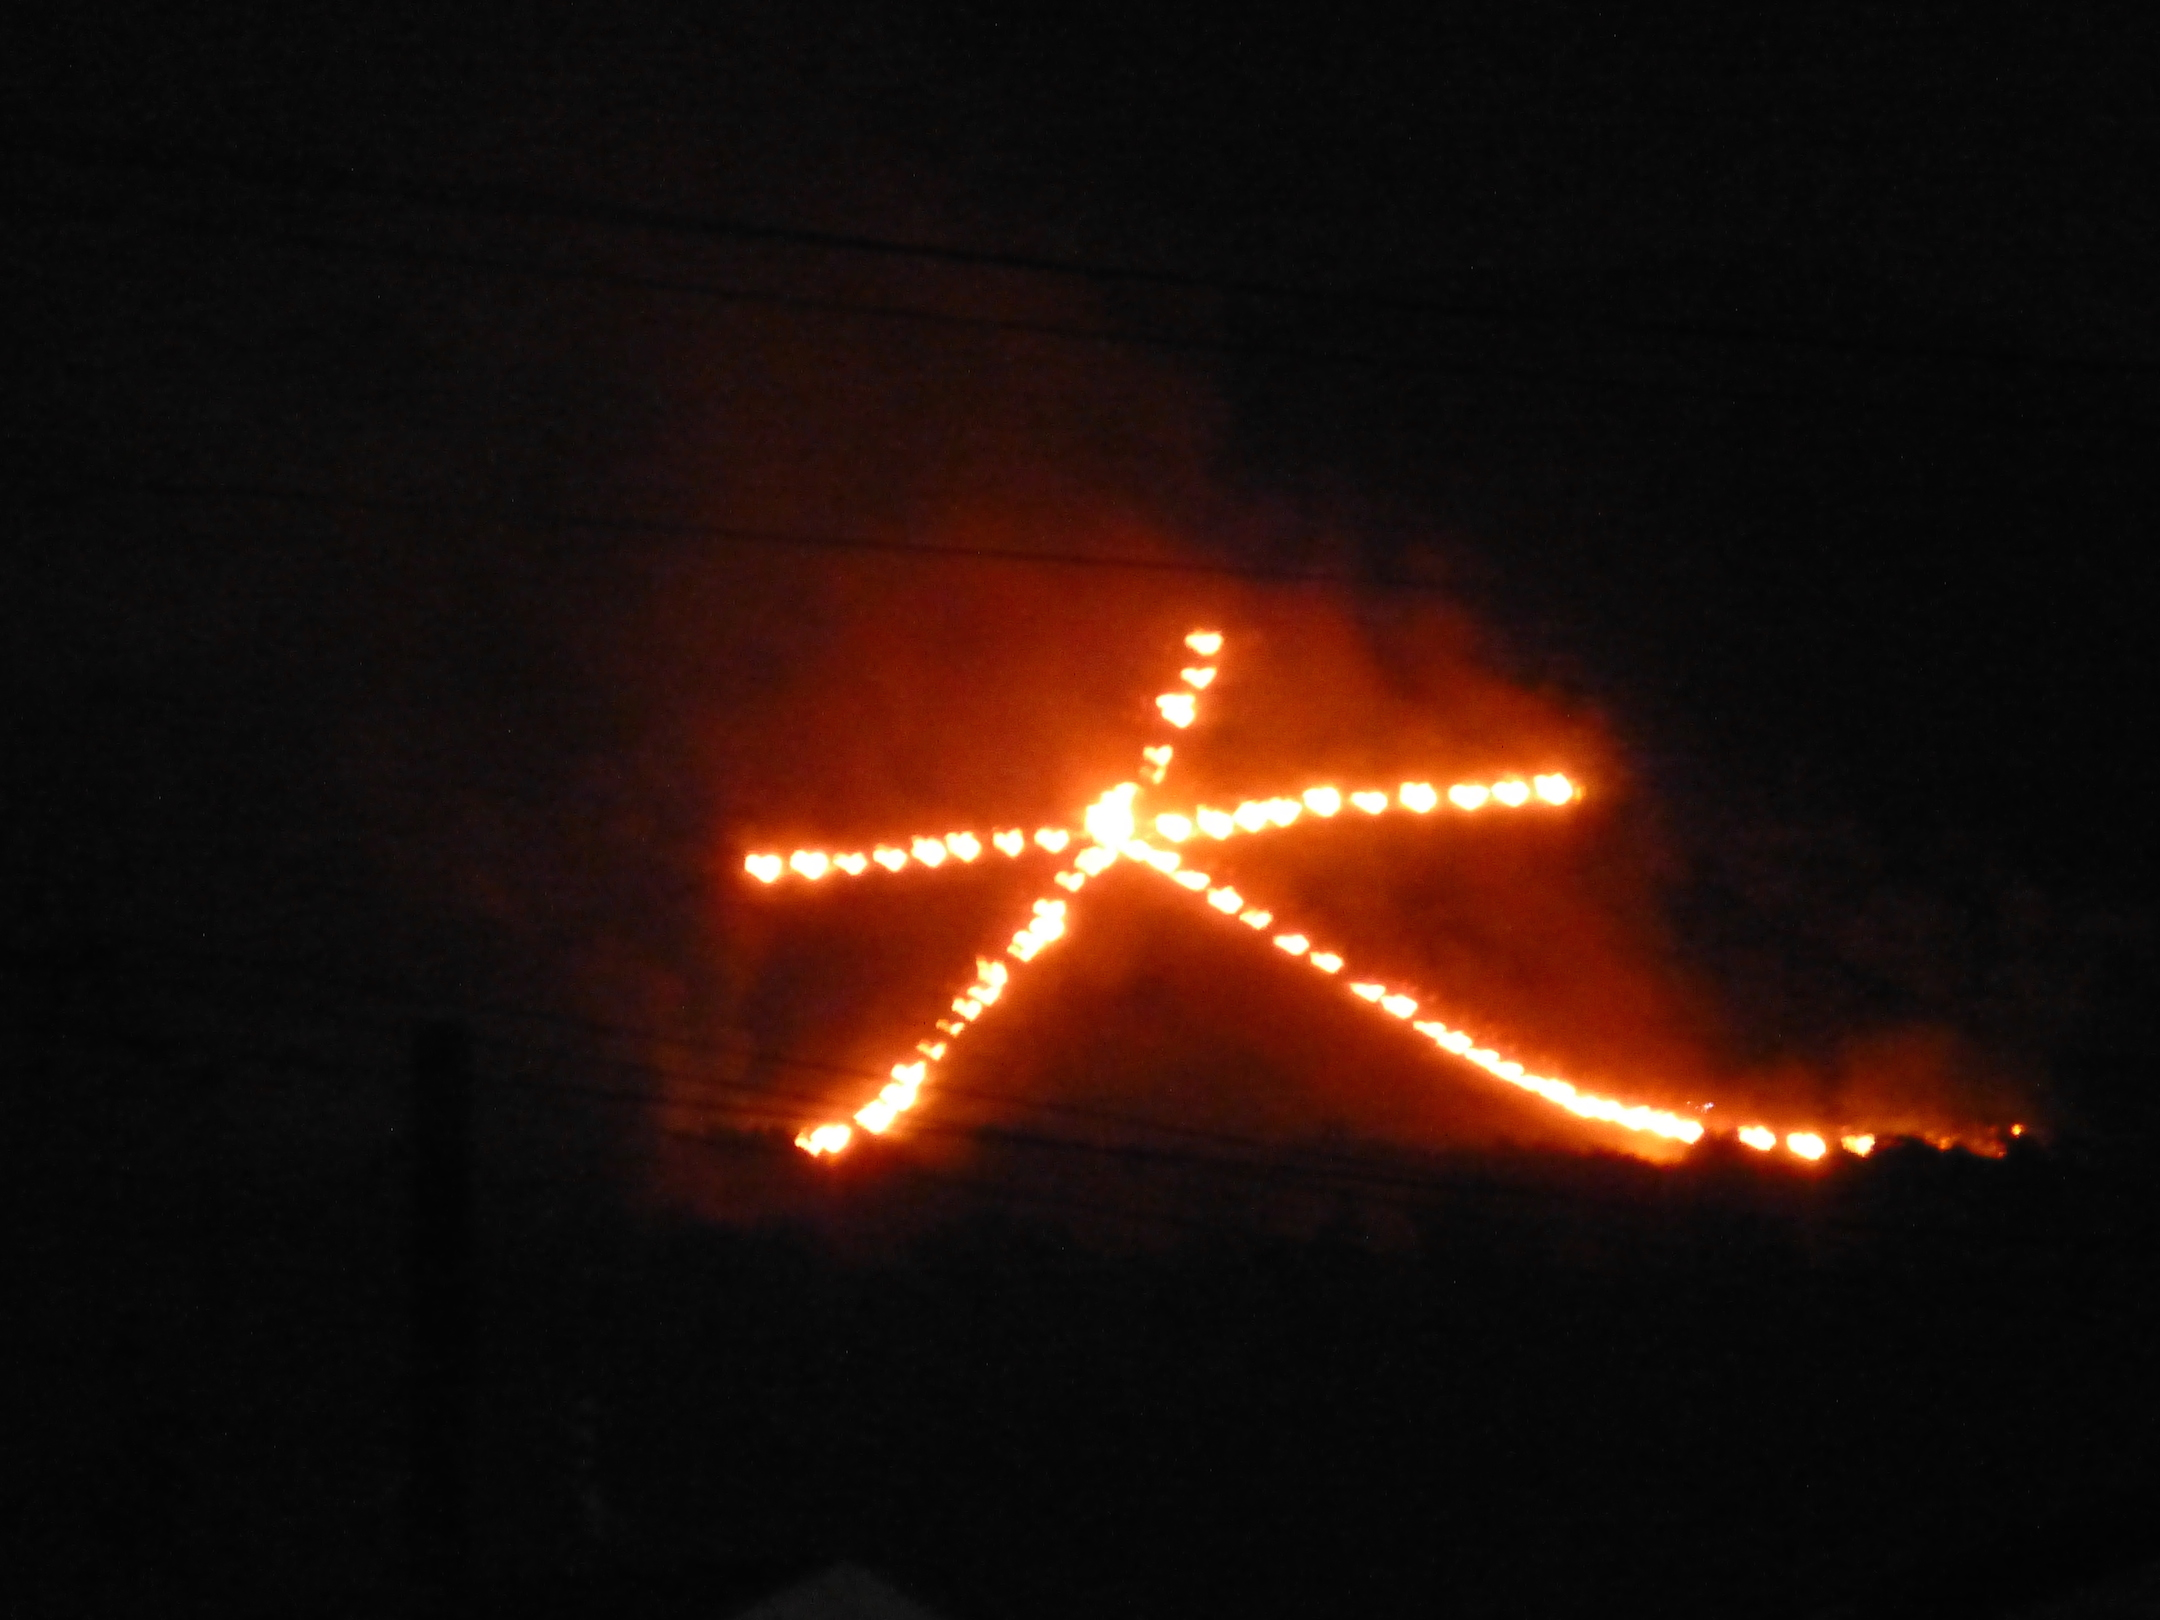
\includegraphics[scale=0.075]
	{figures/jpg/pic03a.jpg}
\end{center}
\end{frame}
%-----------------------------------------------------------------------
\section{Practical Functional programming}

\begin{frame}[fragile]
\frametitle{Practical Functional programming}

\begin{itemize}
\item There is still a lot more to say about the basics: defining
  functions, working with lists, and much more.
\item But let's look now at a complete function program that does
  something useful.
  \begin{itemize}
  \item \emph{Well, at least it's complete.}
  \end{itemize}
\item Introduce some techniques
  \begin{itemize}
  \item How to perform basic text input/output
  \item How to write an interactive program
  \item How to compile and run the program 
  \item How to organise a program
  \end{itemize}
\item Example program: Starman
\end{itemize}

\end{frame}

%-----------------------------------------------------------------------
\begin{frame}[fragile]
\frametitle{Starman}

\begin{itemize}
\item Similar to the traditional hangman game
\item The computer has a word, and the player attempts to guess it
\item On each move:
  \begin{itemize}
  \item The computer displays the word, with known letters shown
    but underscores representing unknown letters
  \item The computer also displays the number of stars you have left
  \item You guess a letter
  \item If correct, the letter is displayed and you keep your stars
  \item If wrong, you lose a star
  \end{itemize}
\item If you complete the word you win; if you run out of stars you
  lose.
\end{itemize}
\end{frame}

%-----------------------------------------------------------------------
\begin{frame}[fragile]
\frametitle{Approach}

We need to
\begin{itemize}
\item Learn how to do basic text I/O
\item Organise the interaction
\item Carry out the calculations
\end{itemize}

We start with some basic techniques used in the program.

\end{frame}

%-----------------------------------------------------------------------
\section{Some basic techniques}

%-----------------------------------------------------------------------
\subsection{Layout}
\begin{frame}[fragile]
\frametitle{Syntax of program structure}

\begin{itemize}
\item Most programming languages (including Haskell) have a
  \emph{block structure} that determines the scoping of names.
\item A common syntax is to enclose the block in braces and to
  separate the elements with semicolon.
\end{itemize}

\begin{verbatim}
  int f (int x, int y)  { 
    int a;
    a = x+y;
    return (a);
   } 
\end{verbatim}

\begin{itemize}
\item The braces/semicolons syntax is redundant, because a
  well-written program is indented.
\item Even worse, the programmer specifies the structure twice:
  once through indentation and again with punctuation.
\item If the indentation and punctuation specify inconsistent
  structure, the program is much harder to read.
\end{itemize}

\end{frame}

%-----------------------------------------------------------------------
\begin{frame}
\frametitle{Haskell uses indentation}

\begin{itemize}
\item Haskell offers a choice: you can use punctuation if you like,
  or you can omit the punctuation and specify the structure through
  indentation.
\item If you aren't using the braces and semicolons, you really
  have to indent the program correctly.
\item There are some detailed rules about how structure is inferred
  from indentation.
\item However, you don't need to learn the rules in detail.  It's
  simpler just to follow the style used in the lecture examples.
\item Occasionally you may see Haskell code that uses punctuation,
  and has random indentation.  But most good Haskell programs use
  the indentation layout.
\end{itemize}

\end{frame}

%-----------------------------------------------------------------------
\subsection{Some standard functions}
\begin{frame}[fragile]
\frametitle{Some standard functions}

The program will use several standard functions, both built-in ones and functions defined in the prelude. LiveScript does not always use the same functions as Haskell, so we provide the \emph{haskell-compat} library to have a greater similarity between.

\end{frame}

%-----------------------------------------------------------------------
\begin{frame}[fragile]
\frametitle{Comparison}

The following operators are used for comparisons; both the ASCII
and typeset versions are shown

\begin{itemize}
\item $x < y$   
\item $x <= y $
\item $x == y $
\item $x >= y $
\item $x > y$   
\end{itemize}

\end{frame}

%-----------------------------------------------------------------------
\begin{frame}[fragile]
\frametitle{$elem$}

\begin{itemize}
\item The function \emph{elem} takes two arguments: a value, and a
  list.  It returns \emph{True} iff the value is an element of the list.
\item You can write \texttt{elem v lst}
\item Equivalently, you can write the function is an infix
  operator: surround it with backward single quotes: \texttt{v `elem` lst}
%\item The Haskell typesetter uses the mathemtatical symbol for
%  element: |v `elem` lst|.
\end{itemize}

\begin{verbatim}
3 `elem` [1,2,3,4] -- > True
6 `elem` [1,2,3,4] -- > False
\end{verbatim}

\end{frame}

%-----------------------------------------------------------------------
\begin{frame}[fragile]
\frametitle{$zip$}

You can zip two lists together into a list of pairs.

\begin{verbatim}
zip [1,2,3] [10.1, 20.2, 30.3] -- > [(1,10.1),(2,20.2),(3,30.3)]
\end{verbatim}

\begin{verbatim}
zip ['a'..'f'] [1..6] -- >
  [('a',1),('b',2),('c',3),('d',4),('e',5),('f',6)]
\end{verbatim}

\begin{verbatim}
zip [4,8] [9,8,7,6,5] -- > [(4,9),(8,8)]
\end{verbatim}

\end{frame}


%-----------------------------------------------------------------------
\subsection{Conditional expressions}

\begin{frame}[fragile]
\frametitle{Conditional expressions}

\begin{itemize}
\item A conditional (if-then-else) expression has the form \texttt{if b
  then e1 else e2}.
\end{itemize}

\begin{verbatim}
if 2<3 then 'a' else 'b'           -- > 'a'
5 * (if 2+2==4 then 6 else 7) + 3  -- > 33
\end{verbatim}

\begin{itemize}
\item As this is an expression, there must always be an \emph{else} clause, otherwise the return value for the \emph{false} branch would not be defined.
\end{itemize}

\end{frame}

%-----------------------------------------------------------------------
\section{Input/output}
\begin{frame}[fragile]
\frametitle{Input/output}

\begin{itemize}
\item Input/output in Haskell uses \emph{IO operations}
\item When there are several IO operations to perform in sequence,
  they are written in a \texttt{do} expression.
\item The entire IO-performing program has type $IO ()$.
\item There is a lot more to say about how this all works, and what
  is really going on---but we'll say it later, not now.
\end{itemize}

\end{frame}
%-----------------------------------------------------------------------
\section{Input/output}
\begin{frame}[fragile]
\frametitle{Input/output}

\begin{itemize}
\item Input/output in LiveScript uses the \emph{Node.js} IO libraries.
\item The important point here is that reading from \emph{stdin} in Node.js is event-based and non-blocking
\item That means that the IO operations are not performed in the order that you write them!
\end{itemize}

\end{frame}

%-----------------------------------------------------------------------
\begin{frame}[fragile]
\frametitle{Hello world in Haskell}

\begin{verbatim}
main = putStrLn "Hello, world!"
\end{verbatim}

\end{frame}
%-----------------------------------------------------------------------
\begin{frame}[fragile]
\frametitle{Performing a sequence of output operations}

This is Prog2.hs:
\begin{verbatim}
main =
  do putStrLn "Some output"
     putStrLn "More output"
     putChar 'x'
\end{verbatim}

\begin{verbatim}
*Main> :load Prog2
[1 of 1] Compiling Main  ( Prog2.hs, interpreted )
Ok, modules loaded: Main.
*Main> main
Some output
More output
x*Main> 
\end{verbatim}

\end{frame}

%-----------------------------------------------------------------------
\begin{frame}[fragile]
\frametitle{Reading a character}

This is Prog3.hs:

\begin{verbatim}
main =
  do putStrLn "Enter a character:"
     c <- getChar
     putStrLn ("You just typed " ++ [c])
\end{verbatim}

\begin{verbatim}
*Main> main
Enter a character:
uYou just typed u
*Main> 
\end{verbatim}

\end{frame}


%-----------------------------------------------------------------------
\begin{frame}[fragile]
\frametitle{Reading a line of text}

\begin{verbatim}
main =
  do putStrLn "Enter a string"
     xs <- getLine
     putStrLn ("You typed <<" ++ xs ++ ">>")
\end{verbatim}

\begin{verbatim}
*Main> main
Enter a string
I typed this text
You typed <<I typed this text>>
*Main> 
\end{verbatim}


\end{frame}

%-----------------------------------------------------------------------
\begin{frame}[fragile]
\frametitle{Summary of IO (so far)}

\begin{itemize}
\item Your program has some name, like \emph{main}.
\item The entire function is a \texttt{do} expression that consists of a
  sequence of ``computations''
\item Each computation may be an output or an input operation
  (there are other possibilities we'll see later)
\item Put each computation on a line by itself, and indent so they
  all start in the same column. (Layout rules!)
\item If a computation is too long to fit on a line, its
  continuation lines need to be indented more deeply.
\end{itemize}

\end{frame}

%-----------------------------------------------------------------------
\begin{frame}[fragile]
\frametitle{Are these really expressions?}

\begin{itemize}
\item A previous lecture claimed that \emph{Haskell has
    expressions, but it doesn't have statements}
  \begin{itemize}
  \item {\redtext But \emph{putStrLn} looks like a print statement, and \emph{getChar}
    looks like a read statement!}
  \end{itemize}
\item True, that's they way they \emph{look}, but actually these
  computations are really expressions, not statements.
  \begin{itemize}
  \item {\redtext Isn't that just playing games with terminology?
    \emph{``Hmmm, if they say that expressions are good and
      statements are bad, then let's just say that our statements
      are actually expressions!''}}
  \end{itemize}
\item Here's one way to look at it:
  \begin{itemize}
  \item The \emph{do} expression with I/O operations looks a lot like C,
    which is useful because {\bluetext your intuition about
      imperative programming will help you to write Haskell.}
  \item Nonetheless, there are some {\bluetext technical
      differences between the Haskell |do| and a sequence of C
      statements.}  We'll examine those later on.  This is
    connected with the statements \emph{\redtext Haskell is pure}
    and \emph{\redtext Haskell has no side effects}.
  \end{itemize}
\end{itemize}

\end{frame}
%-----------------------------------------------------------------------
\section{The Starman program}

\begin{frame}[fragile]
\frametitle{The Starman program}

\begin{itemize}
\item The essence of the game is checking the player's guess, and
  updating the display (the string of underscores shown to the
  player) and the number of stars left.
\item The top level of the game is the interaction with the user.
\end{itemize}

\end{frame}

%-----------------------------------------------------------------------
\subsection{Calculating the result}
\begin{frame}[fragile]

\frametitle{Calculating the result}

The core of the game is for the computer to check the player's guess:

\begin{itemize}
\item We want to know whether the guess was right.  This is a
    \emph{Bool}, so \emph{True} or \emph{False}.
\item We need to update the display, if the guess was right, by
  replacing each underscore where the guessed character appears.
\item Therefore the result type of the function is a pair \emph{(Bool,
  String)}.
\item Now, the checking function
  needs to know:
  \begin{itemize}
  \item The secret \emph{word :: String}.
  \item The current \emph{display :: String}.
  \item The \emph{c::Char} character guessed by the player.
  \end{itemize}
\item Now we can state the signature of the function:
\end{itemize}

\begin{verbatim}
check :: String -> String -> Char -> (Bool,String)
\end{verbatim}

{\bluetext Programming tip: it's useful to work out the type of a
  function first.  This focuses your attention on \emph{what} the
  function is supposed to compute, and \emph{what} data it needs to
  do it.  Only \emph{after} you know what the function is supposed
  to do, should you start implementing it (\emph{how} it calculates
  the result).}

\end{frame}

%-----------------------------------------------------------------------
\begin{frame}[fragile]
\frametitle{Checking the player's guess}

\begin{itemize}
\item The guess is correct if and only if the guess $c$ is an
  element of the list of characters in the target $word$.
  \begin{itemize}
  \item Guess is right if \texttt{c `elem` word}
  \end{itemize}
\item The new display is
  \begin{itemize}
  \item \texttt{[(if x==c then c else y) | (x,y) <- zip word display]]}
  \end{itemize}
\end{itemize}

\begin{verbatim}
check :: String -> String -> Char -> (Bool, String)
check word display c
  = (c `elem` word, [
      if x==c 
          then c 
          else y | (x,y) <- zip word display
          ])
\end{verbatim}

\end{frame}

%-----------------------------------------------------------------------
\section{Interaction with game player}
\begin{frame}[fragile]
\frametitle{Interaction with game player}

\begin{itemize}
\item There are, as always, many ways to organise the program.
\item Our approach:
  \begin{itemize}
  \item A function $move$ that takes the target word and the state
    of the game (the display and number of stars), and decides
    whether the game is over.
  \item If the game isn't over, $move$ will call $tryAgain$ to let the
    player try guessing a letter.
  \item A top level function $starman$ calls $move$ with the right
    initial arguments (this is a trivial function).
  \end{itemize}
\end{itemize}
\end{frame}


%-----------------------------------------------------------------------
\begin{frame}[fragile]
\frametitle{The $move$ function}

\begin{verbatim}
move :: String -> String -> Int -> IO ()
move word display n =
  do if n==0
       then putStrLn "You lose"
       else if word==display
              then putStrLn "You win!"
              else try word display n
\end{verbatim}

\end{frame}

%-----------------------------------------------------------------------
\begin{frame}[fragile]
\frametitle{The $try$ function}

\begin{verbatim}
try word display n =
  do putStrLn (display ++ "  " ++ take n (repeat '*'))
     putStr "  Enter your guess: "
     q <- getChar
     putStrLn ""
     let (correct, display') = check word display q
     let n' = if correct then n else n-1
     move word display' n'
\end{verbatim}
\end{frame}

%-----------------------------------------------------------------------
\begin{frame}[fragile]
\frametitle{The main program}

\begin{verbatim}
starman :: String -> Int -> IO ()
starman word n = move word ['_' | x <- word] n
\end{verbatim}

\end{frame}

\end{document}
